The major usage of \gls{JIT} compilation by \gls{PyExaFMM} is in the construction
of the Octree, including the calculation of the interaction lists for target
boxes, and to accelerate functions for its traversal. The impact of \gls{JIT}
compilation on tree construction is illustrated in figures
(\ref{fig:3_1_octree}) and (\ref{fig:3_1_octree2}), where octrees constructed with
Numpy and Numba together are compared to octrees constructed with just Numpy.
Each tree is constructed to a maximum depth of 5 levels over a unit box
centered at the origin. The construction time is measured against an
the numbers of particles $N$ placed in the tree, which are taken to be
both the sources and the targets. The construction
is repeated five times on each problem size $N$ for statistics, though in both
figure (\ref{fig:3_1_octree}) and (\ref{fig:3_1_octree2}) the error bars, taken
from the standard deviations, are generally too small to see. Figure (\ref{fig:3_1_octree2})
illustrates how the multiplicative speedup offered by \gls{JIT} compilation via
Numba has an optimimum problem size $N$, after which the speedups provided diminish.

\begin{figure}[ht]
    \centering

  {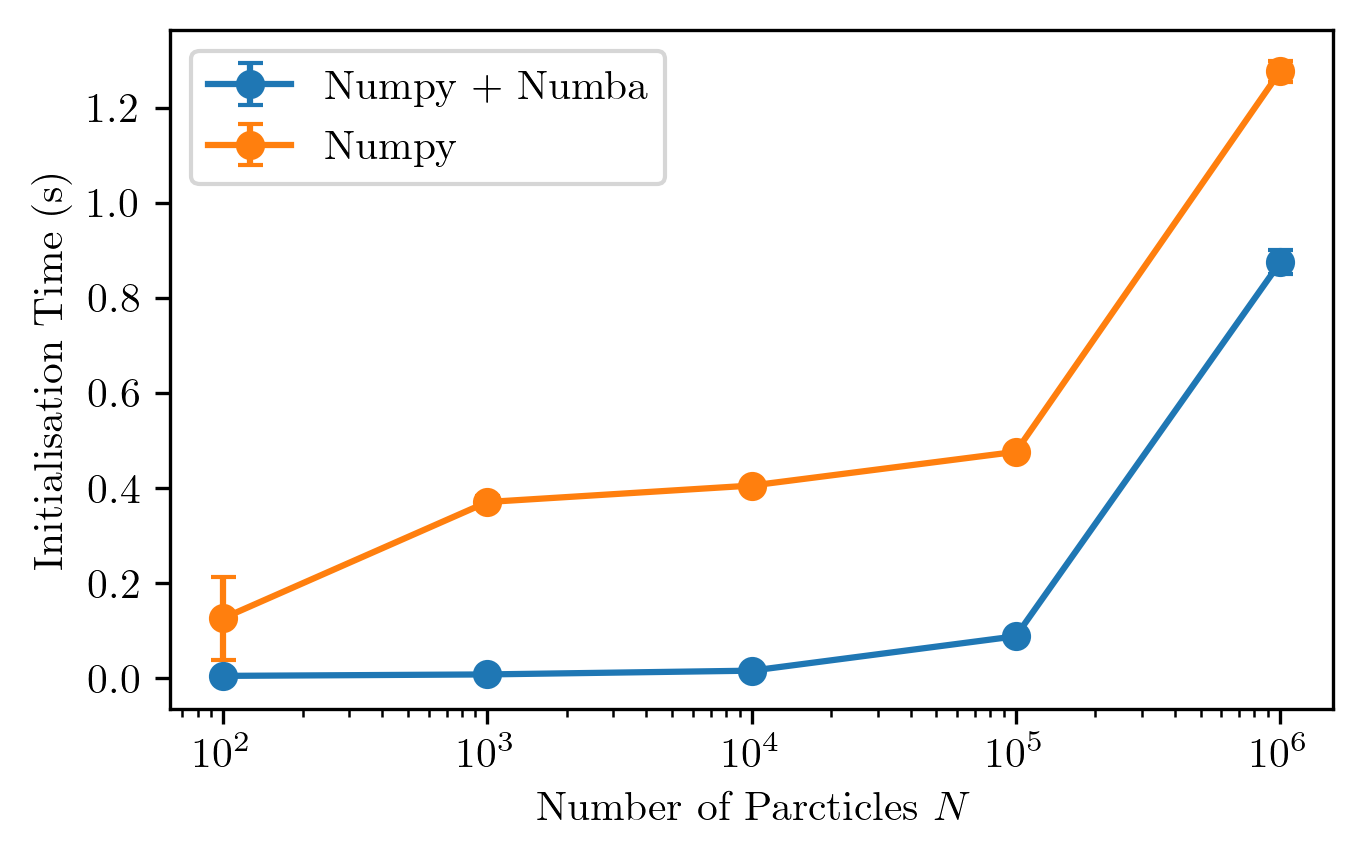
\includegraphics[width=0.9\textwidth]{chapter3/octree.png}}
  \vspace{0pt}
    \caption{
        Comparison of octree initialisation time versus number of particles $N$
        when using Numpy and Numba, to just using Numpy.
    }
    \label{fig:3_1_octree}
\end{figure}

\begin{figure}[ht]
    \centering

  {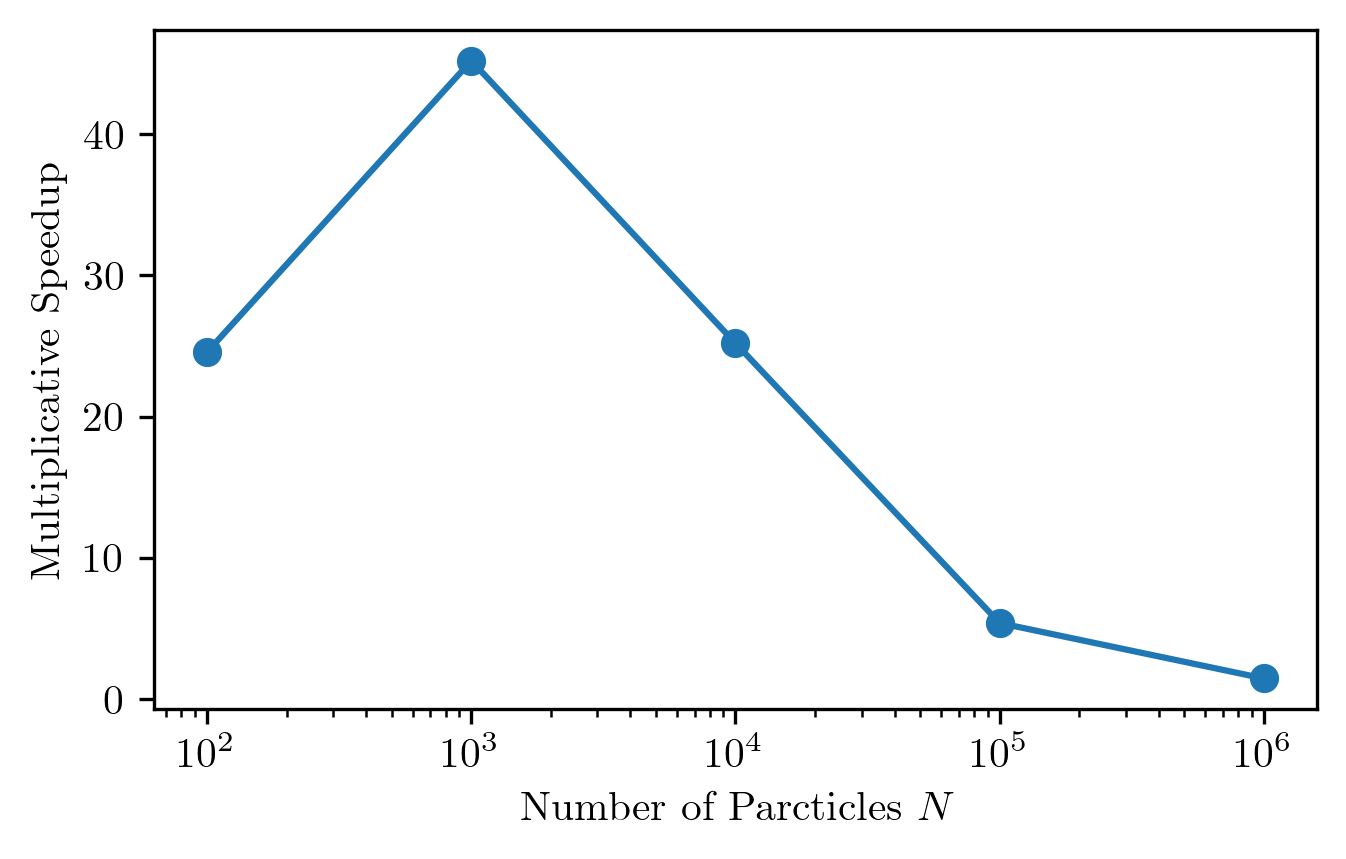
\includegraphics[width=0.9\textwidth]{chapter3/octree2.png}}
  \vspace{0pt}
    \caption{
        Multiplicative speedup offered by using Numba on top of just Numpy for
        initialising octrees.
        The analysis used to calculate the errors is provided in
        Appendix \ref{app:errors}, Section \ref{sec:app_numba}.
    }
    \label{fig:3_1_octree2}
\end{figure}

Table (\ref{table:3_1_jit}) provides timing comparisons for all the octree traversal
functions used in \gls{PyExaFMM} when using Numba and Numpy, or just Numpy alone.
\gls{JIT} compilation relies on a preliminary code analysis, to find optimisations
in the interpreted byte code, this can lead to relatively longer runtimes when
a \gls{JIT} compiled function is first invoked, in comparison to subsequent
invocations. All the calculations in table (\ref{table:3_1_jit}) were run for a
Morton key of 100 placed in a unit box centered at the origin, and were repeated
100 times for statistics. We observe that the preliminary analysis step for
some \gls{JIT} compiled function is so expensive that the mean time for the \gls{JIT}
compiled function is significantly longer than using a function with Numpy alone.
Further investigation is needed to understand exactly why the \gls{JIT} preliminary
analysis takes so much longer for some Numpy based functions than others.

\begin{table}[ht]
    \centering % used for centering table
    \begin{tabular}{c c c} % centered columns (4 columns)
    \hline\hline %inserts double horizontal lines
    Method & Numpy + Numba & Numpy \\ [0.5ex] % inserts table
    %heading
    \hline % inserts single horizontal line
    Get Level of a Key & 280 ns ± 276 ns  & 1.01 µs ± 265 ns \\ % inserting body of the table
    Get Offset of Key & 29.6 µs ± 291 µs & 804 ns ± 324 ns \\
    Remove Offset from a Key & 30.7 µs ± 301 µs & 1.83 µs ± 566 ns \\
    Get Octant of a Key & 23.6 µs ± 231 µs & 2.16 µs ± 2.71 µs \\
    Get Octant Index From Key & 64.4 µs ± 632 µs & 10.7 µs ± 3.82 µs \\
    Get Key From Octant Index & 36.4 µs ± 356 µs & 11.1 µs ± 3.54 µs \\
    Get Octant Index From Cartesian Coordinate & 50.4 µs ± 484 µs & 17.3 µs ± 21 µs \\
    Get Key From Cartesian Coordinate & 2.71 µs ± 1.58 µs & 30.4 µs ± 20.3 µs \\
    Get Box Center From Octant Index & 49.2 µs ± 476 µs & 21.7 µs ± 27.2 µs \\
    Get Box Center From Key & 60.5 µs ± 581 µs & 22.4 µs ± 7.52 µs \\
    Get Parent Key & 29.7 µs ± 292 µs & 2.47 µs ± 546 ns \\
    Get Child Keys & 37.6 µs ± 361 µs & 8.62 µs ± 11.2 µs \\
    Get All Neighbor Keys & 98.4 µs ± 803 µs & 445 µs ± 80.1 µs\\
    Get All Possible Keys In Interaction List & 98.4 µs ± 803 µs & 1.67 ms ± 225 µs \\ [1ex] % [1ex] adds vertical space
    \hline %inserts single line
    \end{tabular}
    \label{table:3_1_jit} % is used to refer this table in the text
    \caption{
        Benchmarking tree traversal functions implemented in \gls{PyExaFMM}.
        Errors are taken from the standard deviation over trials.
        } % title of Table
\end{table}


The loading and saving speeds of a increasingly large files into memory by
HDF5 in comparison to Python's native object serialisation library, Pickle,
are illustrated in figures (\ref{fig:3_1_loadtime}) and (\ref{fig:3_1_savetime})
respectively. Each trial was repeated 5 times with each file size for statistics.
The multiplicative speedups for loading and saving using HDF5 are illustrated
in figures (\ref{fig:3_1_loadtime_speedup}) and (\ref{fig:3_1_savetime_speedup})
respectively.

We observe that the speedup offered by HDF5 for loading and saving
data is approximately constant over file size. The reasons for this are due to the underlying
techniques used by each method. Roughly speaking, HDF5 stores raw numeric data
alongside a header file describing its dimensions, as a contiguous byte stream
on disk which allows for optimised methods to quickly search and retrieve data
\cite{collette2013python}. Object serialisation is designed to work with arbitrary
Python objects, raw numeric data is not stored, rather it is first compressed
into an intermediate representation, that results in a byte stream which is then
stored on disk. This data is stored alongside the metadata for the object, such
as it's initialisation code, and even any dependent objects it may have. The
intermediate representation allows any objects to be serialised in the same
manner \cite{pickle}.

\begin{figure}
    \centering

  {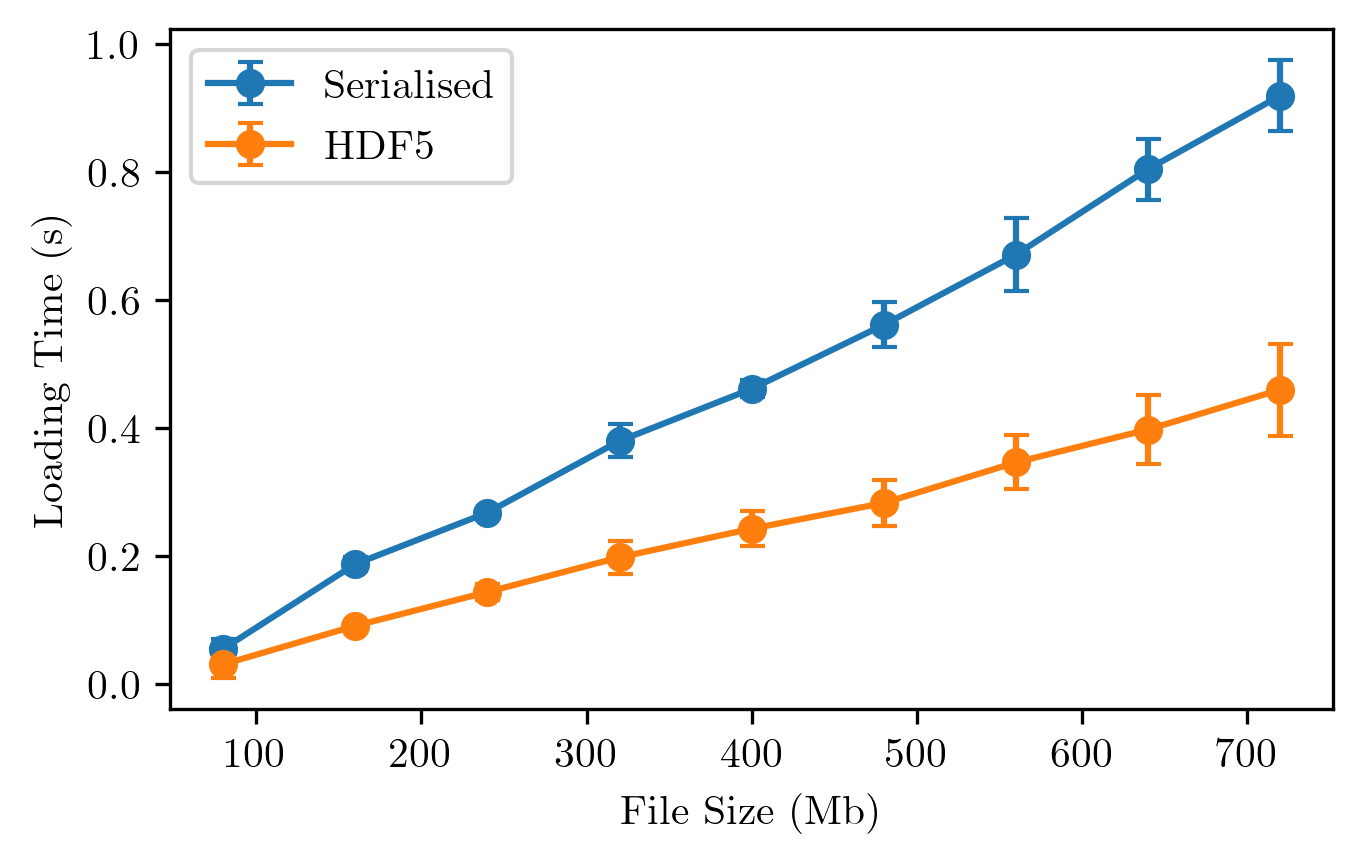
\includegraphics[width=0.9\textwidth]{chapter3/loadtime.png}}
  \vspace{0pt}
    \caption{
        Loading times versus File Size comparing object serialisation to HDF5.
    }
    \label{fig:3_1_loadtime}
\end{figure}


\begin{figure}
    \centering

  {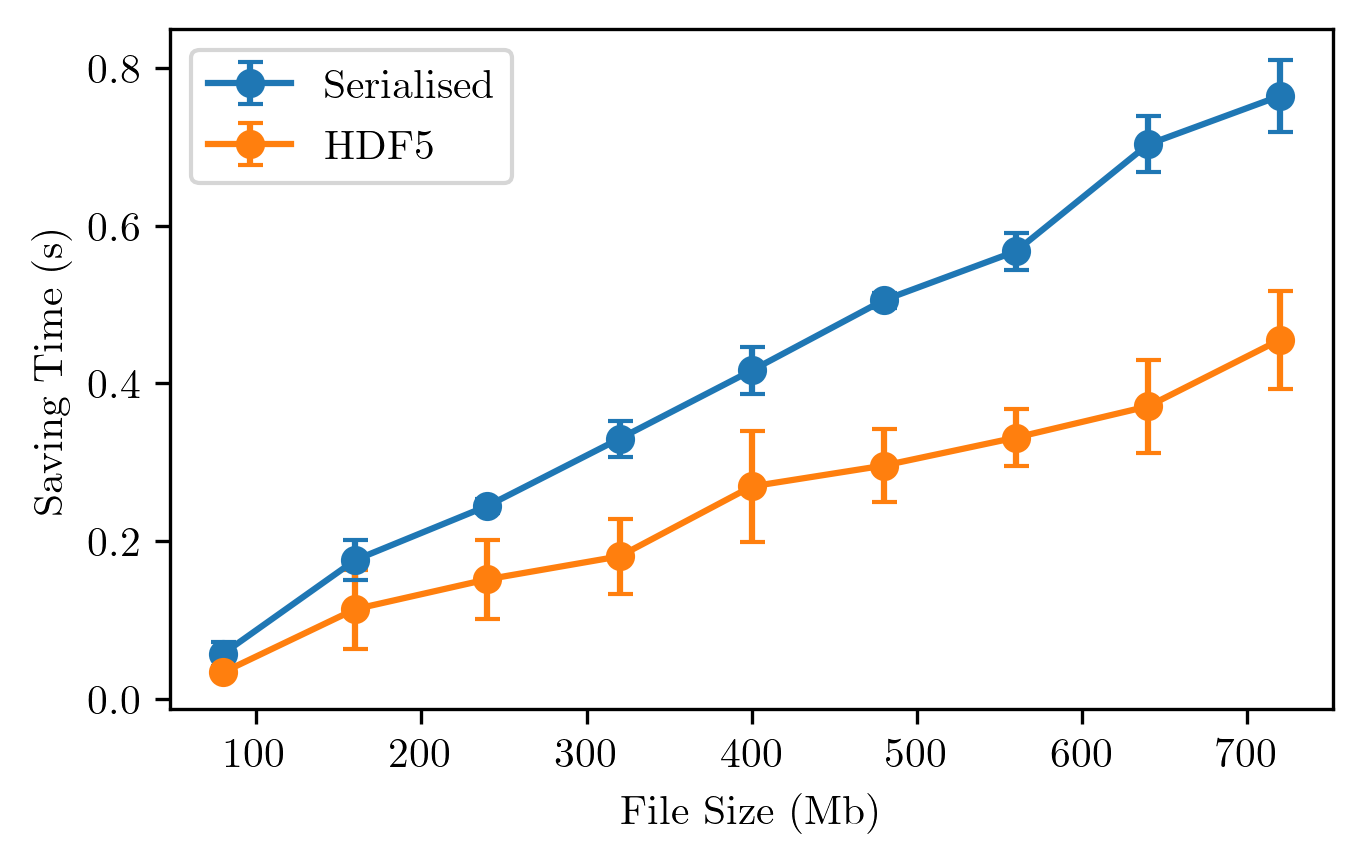
\includegraphics[width=0.9\textwidth]{chapter3/savetime.png}}
  \vspace{0pt}
    \caption{
        Saving times versus File Size comparing object serialisation to HDF5.
    }
    \label{fig:3_1_savetime}
\end{figure}


\begin{figure}
    \centering

  {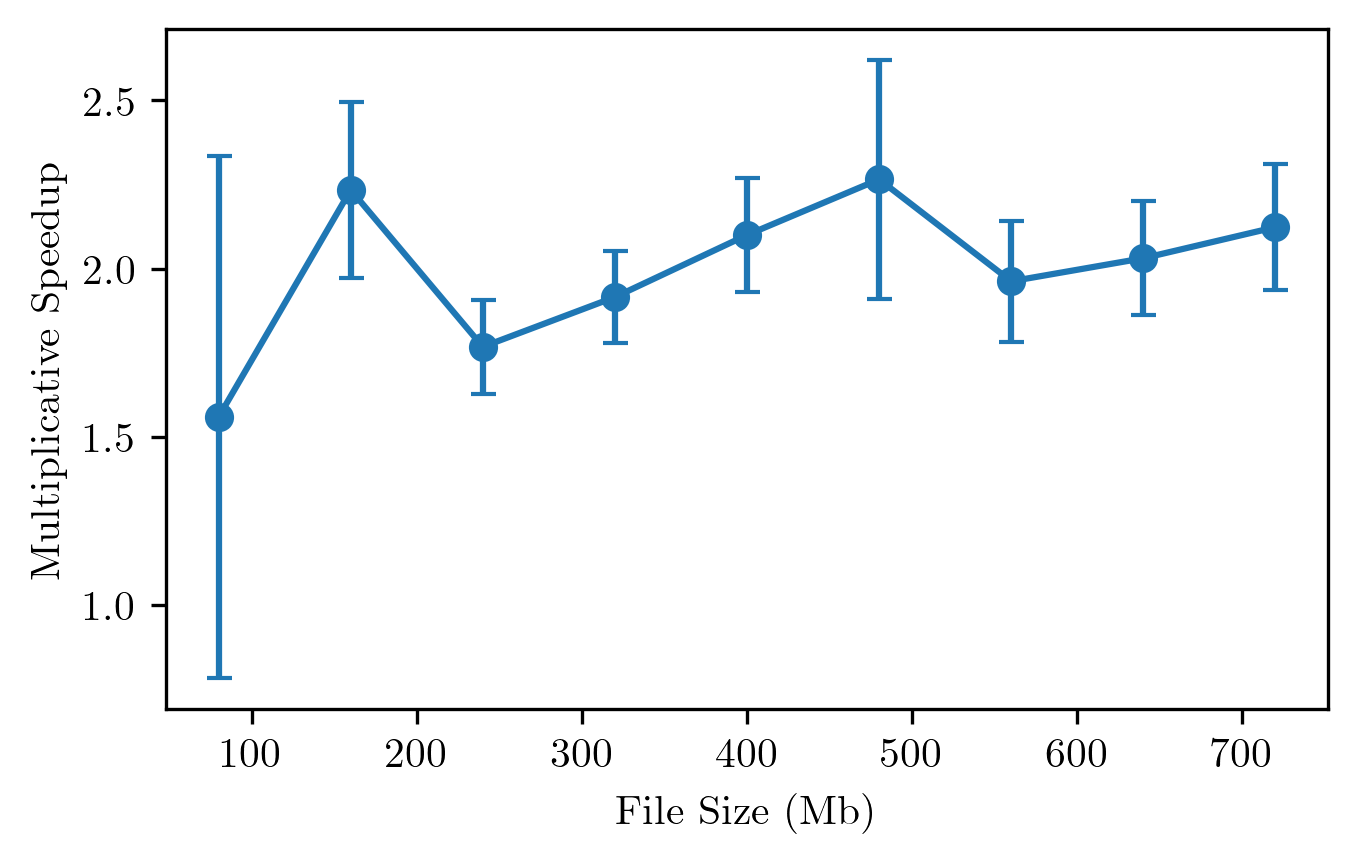
\includegraphics[width=0.9\textwidth]{chapter3/loadtime_speedup.png}}
  \vspace{0pt}
    \caption{
        The multiplicative speedup offered by HDF5 over object serialisation
        as a function of file size for loading files.
        The analysis used to calculate the errors is provided in
        Appendix \ref{app:errors}, Section \ref{sec:app_numba}.
    }
    \label{fig:3_1_loadtime_speedup}
\end{figure}


\begin{figure}
    \centering

  {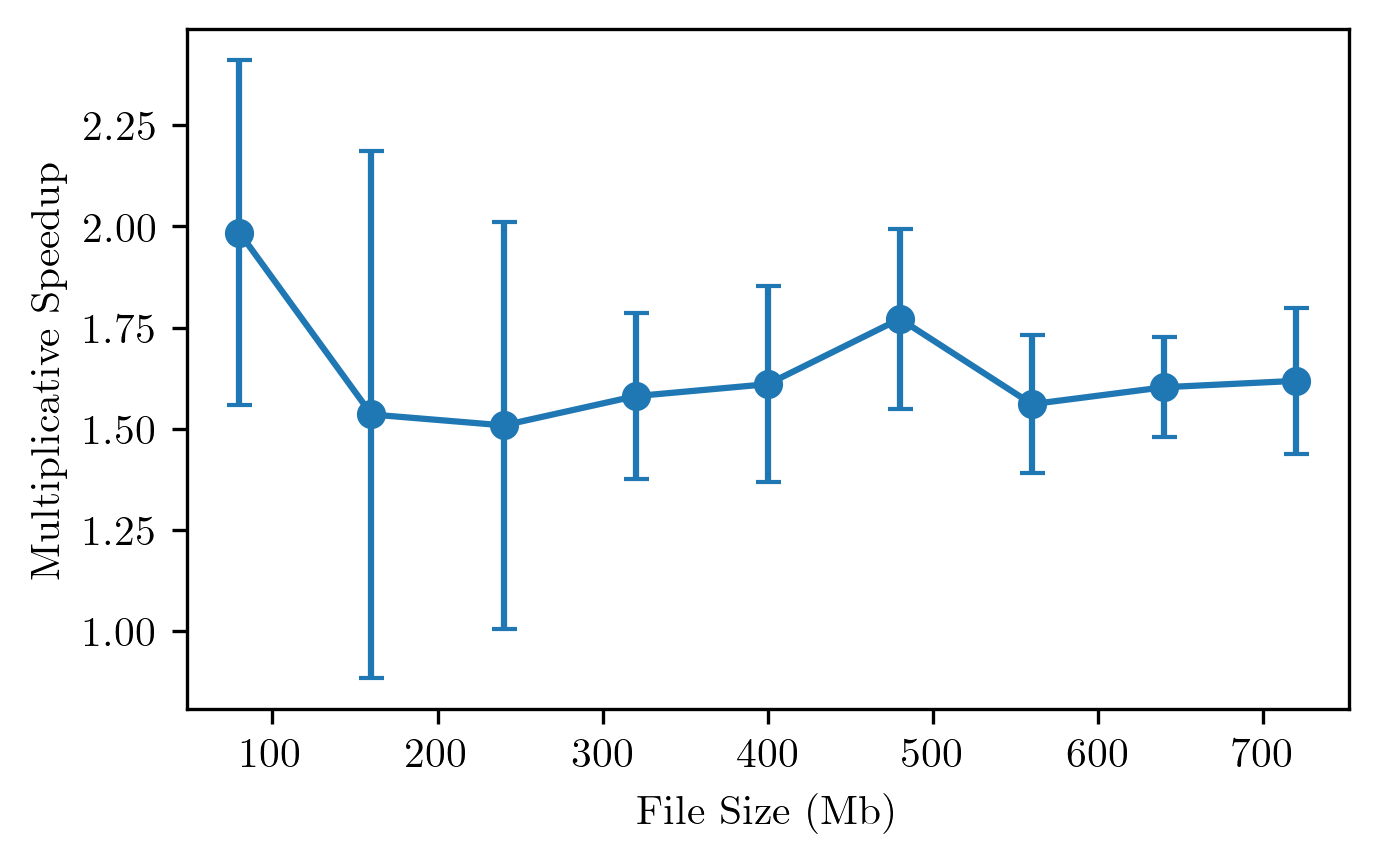
\includegraphics[width=0.9\textwidth]{chapter3/savetime_speedup.png}}
  \vspace{0pt}
    \caption{
        The multiplicative speedup offered by HDF5 over object serialisation
        as a function of file size for saving files.
        The analysis used to calculate the errors is provided in
        Appendix \ref{app:errors}, Section \ref{sec:app_numba}.
    }
    \label{fig:3_1_savetime_speedup}
\end{figure}


The effect of multiprocessing on operator matrix precomputations is
illustrated in figure (\ref{fig:3_1_multiproc}). Here, we solve
for operator matrices of the model electrostatic problem in three dimensions
(\ref{eq:electrostatic_paradigm}), using a tree with a maximum depth of 3 levels,
and 1000 randomly distributed particles in a unit cube, varying the number of
processor cores accessible to the script. These are taken to be
both sources and targets. Unit charges are placed on each source particle, and
all relevant surfaces are calculated to order $p=2$, therefore discretised
with 8 quadrature points (\ref{eq:2_2_quadrature_points}). The parameters for
the relative sizes of different surfaces are the same as those provided
in Chapter \ref{chpt:2_strategy_for_practical_implementation},
Section \ref{sec:2_3_operator_caching}. The speedup offered by increasing the
number of processor cores is non-linear, this is indicative of a communication
overhead, and the fact that multiprocessing has been implemented to a very
basic degree with the required data being copied to each process, even if very large.

\begin{figure}[ht]
    \centering

  {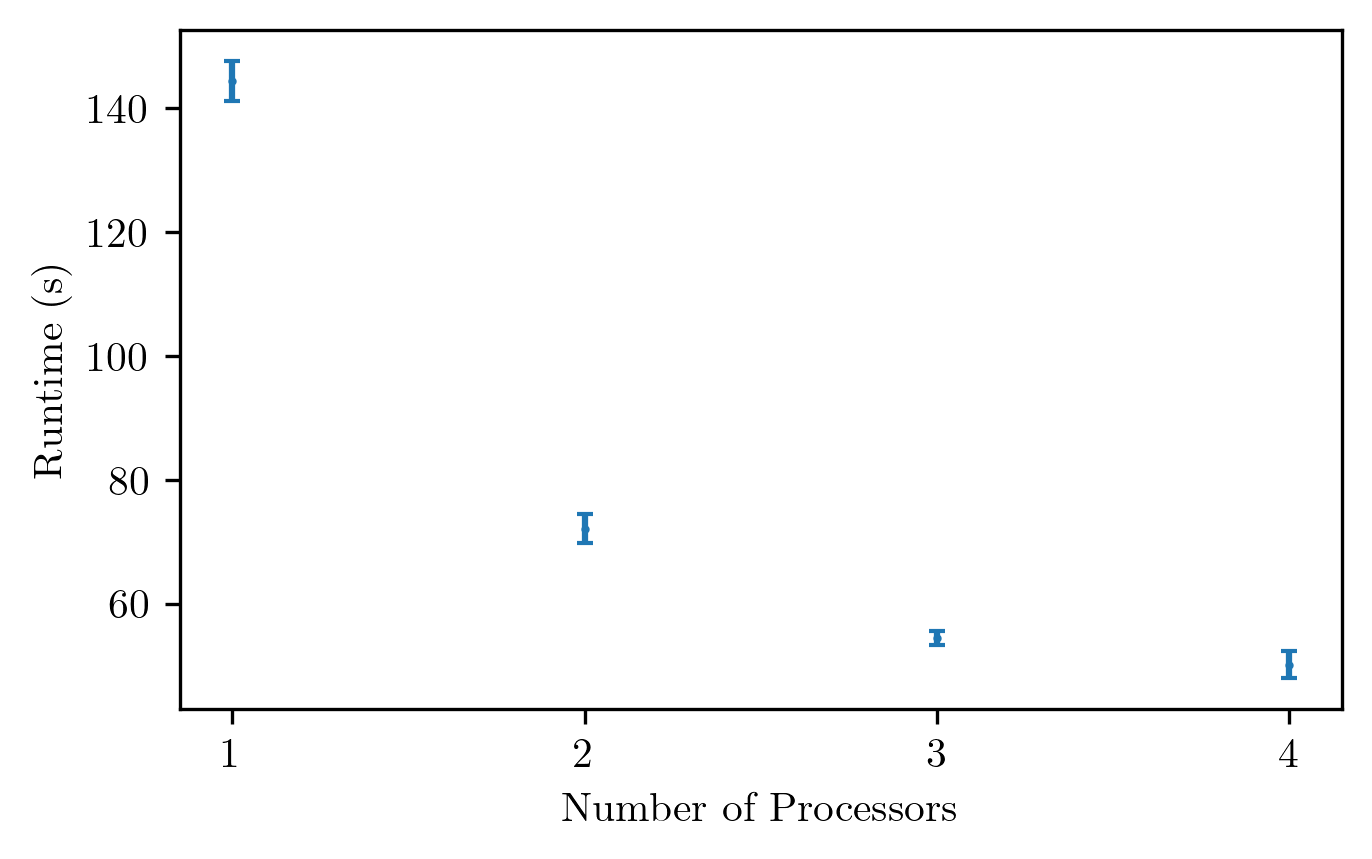
\includegraphics[width=0.9\textwidth]{chapter3/multiproc.png}}
  \vspace{0pt}
    \caption{Runtime versus number of processors used for operator precomputations
    for the model problem (\ref{eq:electrostatic_paradigm}). Error bars are
    plotted using standard deviation.
    }
    \label{fig:3_1_multiproc}
\end{figure}

We benchmark the algorithm run time in comparison to direct computation in figure
(\ref{fig:3_1_complexity}), with same octree parameters as used for benchmarking
the operator precomputation, but with an increasing number of target and source
particles $N$ for our model problem (\ref{eq:electrostatic_paradigm}). The
calculations are run three times for each problem size for statistics.
Assuming a power relationship between run time $t$ and problem size $N$,

\begin{equation}
    t = N^x
\end{equation}

where $x$ is unknown, taking logarithms allows one to apply least squares fitting
to fit a linear relationship to,

\begin{equation}
    \log(t) = x \log(N)
\end{equation}

computing the value of $x$ from the gradient. Performing this calculation for the
results from the \gls{FMM} and direct approaches we report $x=1.14$ (2 d.p) for
the FMM, and $x=1.98$ (2 d.p) for the direct method. This implies an approximate
asymptotic complexity of $O(N)$, and $O(N^2)$ for the \gls{FMM} and direct methods
respectively in line with what is expected, with the limitation that this has
been tested on relatively small inputs of only $O(10^3)$ particles.

\begin{figure}[ht]
    \centering

  {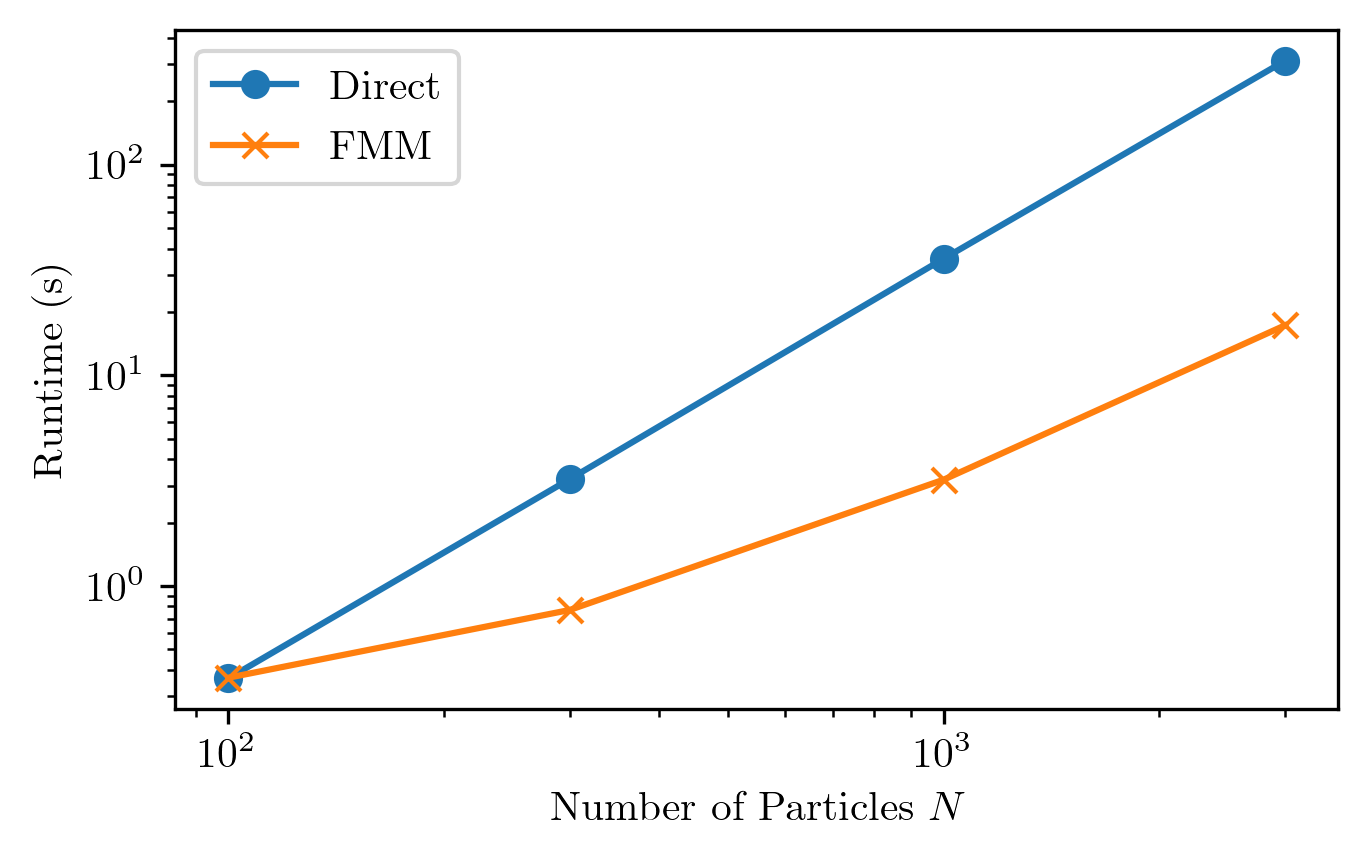
\includegraphics[width=0.9\textwidth]{chapter3/complexity.png}}
  \vspace{0pt}
    \caption{
        Runtime versus problem size to solve the model problem
        (\ref{eq:electrostatic_paradigm}) using direct calculations and
        \gls{PyExaFMM}.
    }
    \label{fig:3_1_complexity}
\end{figure}

We report that with a simulation with the above octree and
$N=3000$ takes $17.1 \pm 0.2$ s, over the three runs with
error calculated from standard deviation and reported to 1 s.f. From correspondence
with the authors of ExaFMM-T, we can report their corresponding benchmark figure,
calculated on a 14 Core Intel i9-7940X \gls{CPU} with $N=10^6$ particles
randomly distributed in a unit cube, it takes 0.52 s to perform a $p=4$ degree
computation, including tree construction but excluding the
operator precomputations, in single precision \cite{exafmm}. Time limitations for this project
makes it difficult to perform comparisons using equivalent hardware, however
disparities in hardware are unlikely to explain the magnitude of superiority
of ExaFMM-t's performance in comparison to \gls{PyExaFMM}.

ExaFMM-T implements a range of optimisations which represent future avenues
of software development for \gls{PyExaFMM}. Specifically, they distribute the
\gls{P2P} and \gls{M2L} operations on \gls{GPU}s, as discussed in Chapter
\ref{chpt:2_strategy_for_practical_implementation},
Section \ref{sec:2_3_operator_caching}, as well as using \gls{OpenMP} to share
precomputed surfaces across processes in the operator precomputations.
\gls{PyExaFMM} does not distribute any calculations on \gls{GPU}s, and
wastefully copies surface data to each process for the operator precomputations.
Furthermore, ExaFMM-t optimises the application of the kernel function,
firstly by the inverse operation in (\ref{eq:electrostatic_paradigm}) using a Newton
iteration to approximate $x = 0.5x(w-ax^2)$ to approximate $x \approx a ^{-1/2}$,
the computation for which highly-optimised implementations exist
\cite{Lomont:2003, sqrt}. Secondly \textbf{\gls{AVX}} vectorisation is used
to apply the kernel function. Roughly speaking, \gls{AVX} vectorisation allows
for parallel execution of \gls{SIMD} type instructions in a \gls{CPU}. With similar
optimisations, PVFMM is able to report a 3.8 times multiplicative speed up, in
comparison to naive applications of the Laplace kernel \cite{Malhotra:2015:CCP}.

